\chapter{Introducción}
\label{chap:introduccion}

\section{Contexto: Vulnerabilidad Energética en Zonas Remotas}

La seguridad energética en regiones remotas es un desafío global reconocido en la literatura académica reciente. Un estudio de 2025 sobre islas y regiones aisladas identifica que estas zonas enfrentan vulnerabilidades únicas: dependencia de suministros externos, infraestructura logística precaria, y exposición a disrupciones climáticas y geopolíticas\cite{EnergyIslanded2025}. Estas regiones operan, paradójicamente, en un régimen de alta demanda específica (consumo per cápita elevado debido a condiciones climáticas extremas) y baja redundancia de suministro (cadenas logísticas lineales sin alternativas).

La literatura sobre resiliencia de cadenas de suministro distingue entre \textit{vulnerabilidad} (exposición a amenazas) y \textit{resiliencia} (capacidad de absorción y recuperación)\cite{Ponomarov2009,Christopher2004}. Las cadenas de suministro energético en zonas remotas exhiben alta vulnerabilidad estructural: topologías lineales, largas distancias de transporte, y dependencia de infraestructura crítica (puentes, pasos fronterizos, rutas únicas)\cite{Sheffi2005}. Cuando estas cadenas enfrentan disrupciones prolongadas, el impacto social es inmediato y severo: pérdida de calefacción en climas extremos, interrupción de servicios esenciales (hospitales, escuelas), y riesgo de colapso de actividades económicas locales.

Un caso paradigmático de esta realidad se encuentra en la Patagonia chilena, específicamente en la Región de Aysén.

\section{El Caso de la Región de Aysén: Un Sistema en el Límite}

La Región de Aysén se ubica en la Patagonia chilena, a más de 1,600 km al sur de Santiago. Con 103,000 habitantes dispersos en 108,494 km² (densidad: 0.95 hab/km²), la región enfrenta condiciones que la convierten en un laboratorio natural para el estudio de vulnerabilidad energética. El clima patagónico impone demandas energéticas extremas: temperaturas invernales de hasta $-20°$C, precipitaciones anuales superiores a 3,000 mm en zonas cordilleranas, y vientos constantes de más de 100 km/h.

El suministro de GLP a la región depende de una única vía de acceso terrestre desde Argentina: la Ruta 7, que conecta las plantas de Cabo Negro y Neuquén (Argentina) con Coyhaique a través de un trayecto de aproximadamente 1,400 km. Como muestra la Figura~\ref{fig:mapa-aysen}, el 86\% de este trayecto transcurre en territorio argentino, atravesando el paso fronterizo Huemules antes de ingresar a Chile. Esta dependencia de una infraestructura lineal sin redundancia configura una vulnerabilidad estructural crítica del sistema de suministro.

% Mapa de la región (TikZ)
\begin{figure}[htbp]
    \centering
    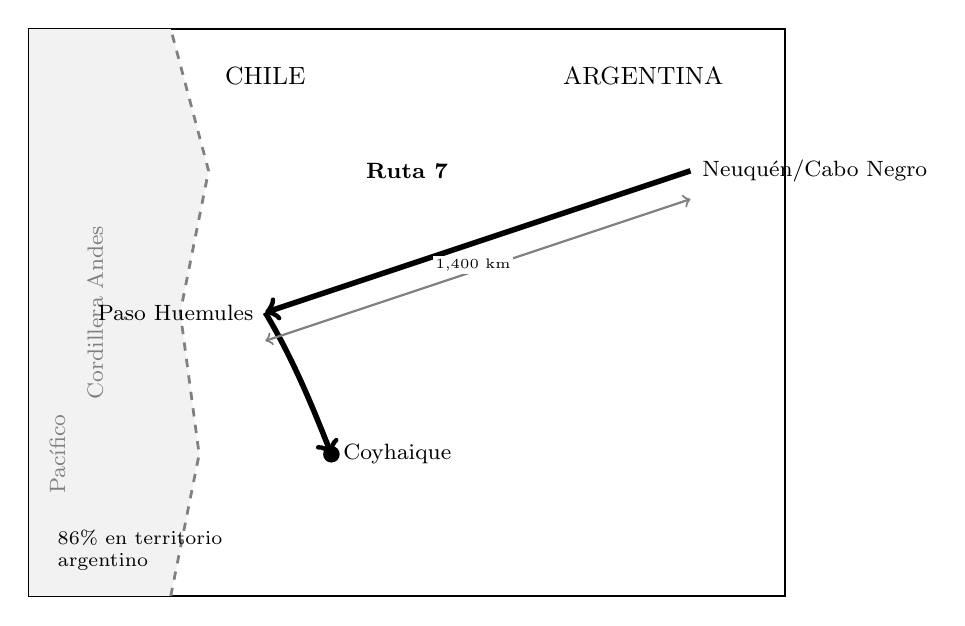
\begin{tikzpicture}[
        font=\small,
        scale=1.2
    ]
        % Marco del mapa
        \draw[draw=black, line width=1pt] (0,0) rectangle (8,6);

        % Cordillera de los Andes
        \fill[gray!10]
            (0,0) -- (1.5,0) -- (1.8,1.5) -- (1.6,3) -- (1.9,4.5) -- (1.5,6) -- (0,6) -- cycle;
        \draw[gray, line width=1pt, dashed]
            (1.5,0) -- (1.8,1.5) -- (1.6,3) -- (1.9,4.5) -- (1.5,6);
        \node[gray, rotate=90, font=\footnotesize]
            at (0.7,3) {Cordillera Andes};

        % Países
        \node[font=\small] at (6.5,5.5) {ARGENTINA};
        \node[font=\small] at (2.5,5.5) {CHILE};

        % Ruta 7
        \draw[black, line width=2pt, ->]
            (7,4.5) node[right, font=\footnotesize] {Neuquén/Cabo Negro}
            .. controls (5.5,4) and (4,3.5) ..
            (2.5,3) node[left, font=\footnotesize, text width=2cm, align=right] {Paso Huemules};

        \draw[black, line width=2pt, ->]
            (2.5,3) .. controls (2.8,2.5) and (3,2) ..
            (3.2,1.5) node[right, font=\footnotesize] {Coyhaique};

        % Coyhaique (punto)
        \fill[black] (3.2,1.5) circle (2.5pt);

        % Distancia
        \draw[<->, gray, line width=0.8pt]
            (7,4.2) -- (2.5,2.7);
        \node[fill=white, font=\tiny, inner sep=1pt] at (4.7,3.5) {1,400 km};

        % Océano
        \node[gray, font=\footnotesize, rotate=90] at (0.3,1.5) {Pacífico};

        % Etiqueta ruta
        \node[font=\footnotesize\bfseries] at (4,4.5) {Ruta 7};

        % Leyenda
        \node[anchor=north west, font=\scriptsize, text width=3cm, align=left]
            at (0.2,0.8) {
                86\% en territorio\\
                argentino
            };

    \end{tikzpicture}
    \caption{Ubicación geográfica de la Región de Aysén y la Ruta 7. Fuente: Elaboración propia con datos de~\cite{CIEP2025}.}
    \label{fig:mapa-aysen}
\end{figure}

En este contexto, el Gas Licuado de Petróleo (GLP) no es una commodity energética opcional: es el único combustible disponible para calefacción residencial, cocción de alimentos, y agua caliente sanitaria para el 100\% de la población urbana y el 78\% de la población rural\cite{CIEP2025}. Con un consumo per cápita de 27.25 Gcal/año (65\% superior a la media nacional de 16.5 Gcal), la región opera en un régimen de alta intensidad energética sin alternativas de corto plazo. No existe red de gas natural, la leña enfrenta restricciones ambientales crecientes, y la electricidad tiene costos prohibitivos para calefacción.

\subsection{Anatomía de una Vulnerabilidad Crítica}

El sistema de suministro presenta tres características que, en combinación, generan una vulnerabilidad sistémica:

\textbf{1. Dependencia absoluta de fuentes externas.} La totalidad del GLP consumido en Aysén se importa desde Argentina vía terrestre. No existe producción local ni alternativas de abastecimiento marítimo o aéreo\cite{CIEP2025}. Esta dependencia del 100\% configura lo que en la literatura de resiliencia se denomina un \textit{single point of failure}: un elemento cuya falla compromete la operación completa del sistema\cite{Sheffi2005}.

\textbf{2. Infraestructura logística lineal sin redundancia.} El GLP transita 1,400 km desde las plantas de Cabo Negro o Neuquén (Argentina) hasta Coyhaique por la Ruta 7, atravesando el paso fronterizo Huemules. El 86\% del trayecto transcurre en territorio argentino\cite{CIEP2025}. No existen rutas alternativas: la geografía patagónica (Cordillera de los Andes, glaciares, fiordos) imposibilita la construcción de infraestructura vial adicional sin inversiones multimillonarias. Esta topología lineal contrasta con la recomendación de la literatura de gestión de riesgos, que enfatiza la importancia de redundancia y diversificación en cadenas de suministro críticas\cite{Christopher2004,Lucker2025}.

\textbf{3. Exposición a disrupciones recurrentes y prolongadas.} La Ruta 7 enfrenta cierres por:
\begin{itemize}
    \item \textbf{Nevadas y derrumbes:} El paso Huemules (1,200 m.s.n.m.) experimenta nevadas que cierran la ruta con frecuencia "casi segura" (Nivel 4 de probabilidad: al menos 1 vez cada 3 meses)\cite{CIEP2025}.
    \item \textbf{Conflictos sociales en Argentina:} El informe CIEP documenta disrupciones de hasta 21 días consecutivos durante el conflicto social de Argentina en 2021, cuando cortes de ruta impidieron el tránsito de camiones.
\end{itemize}

Estudios recientes sobre vulnerabilidad energética identifican que la combinación de dependencia geográfica, exposición a riesgos climáticos, y fragilidad institucional (en este caso, dependencia de la estabilidad política de un país vecino) constituye el escenario de mayor riesgo para la seguridad energética\cite{EnergySecurity2025}.

\subsection{El Gap Estructural: 8.2 Días vs. 21 Días}

El sistema opera con tres distribuidores (Abastible, Lipigas, Gasco) que almacenan 431 toneladas en Coyhaique. Contra una demanda promedio de 52.5 TM/día (calibrada al mes de mayor consumo invernal), esta capacidad proporciona una autonomía teórica de 8.2 días:

\begin{equation}
\text{Autonomía} = \frac{431 \text{ TM}}{52.5 \text{ TM/día}} = 8.2 \text{ días}
\label{eq:autonomia-actual}
\end{equation}

Esta autonomía es apenas superior al lead time nominal de entrega (6 días). Cuando ocurre una disrupción que extiende el lead time más allá de 2 días adicionales, el sistema entra en déficit. Las disrupciones documentadas alcanzan hasta 21 días\cite{CIEP2025}, generando un gap estructural de $8.2 - (6 + 21) < 0$ días. Matemáticamente, el sistema opera en régimen de \textit{subcapacidad crónica}.

\subsection{Impacto Humano y Social}

Cuando el sistema falla, las consecuencias no son abstractas: 103,000 personas quedan sin calefacción en temperaturas bajo cero, hospitales enfrentan riesgo de interrupción de servicios críticos (esterilización, agua caliente), y la actividad económica (hoteles, restaurantes, comercio) se paraliza. Un estudio sobre energía en comunidades remotas de la Patagonia chilena documenta que la vulnerabilidad energética tiene efectos cascada: cuando falla el suministro, las comunidades deben improvisar soluciones informales (quema de desechos, uso de combustibles contaminantes) que generan riesgos adicionales para la salud y el medio ambiente\cite{EnergyPuertoEden2024}.

La gestión actual de crisis es reactiva y manual: ante una disrupción, la autoridad regional "llama a todas las empresas, construye un Excel y saca una foto de cuánta disponibilidad de combustible hay" (Tarik Laibe, Seremi de Energía, comunicación personal, 11 de junio 2025). No existe capacidad de análisis prospectivo ni cuantificación de escenarios.

\section{Pregunta de Investigación y Contribución}

En este contexto, surge una pregunta de ingeniería crítica: ¿cómo cuantificar la resiliencia del sistema bajo diferentes escenarios de inversión y mitigación de disrupciones? Específicamente, la empresa Gasco propone una inversión de \$1.5 millones USD para expandir su capacidad de almacenamiento de 41 TM a 291 TM, elevando la capacidad total del sistema de 431 TM a 681 TM (Propuesta 10.4)\cite{CIEP2025}. Esta inversión aumentaría la autonomía teórica a 13 días.

Sin embargo, la teoría de gestión de inventarios bajo incertidumbre establece que la resiliencia no depende solo de la capacidad total, sino también de la variabilidad del lead time\cite{Silver1998,Chopra2019}. La ecuación del stock de seguridad evidencia esta relación:

\begin{equation}
SS = Z_{\alpha} \sqrt{\bar{LT}\sigma_D^2 + \bar{D}^2\sigma_{LT}^2}
\label{eq:stock-seguridad}
\end{equation}

donde $SS$ es el stock de seguridad necesario, $Z_{\alpha}$ es el factor de servicio para un nivel de servicio deseado, $\bar{D}$ y $\sigma_D$ son la media y desviación estándar de la demanda, y $\bar{LT}$ y $\sigma_{LT}$ son la media y desviación estándar del lead time. En Aysén, la demanda es relativamente estable ($\sigma_D$ bajo) pero el lead time es altamente volátil ($\sigma_{LT}$ alto debido a disrupciones). La ecuación simplificada revela que $SS \propto \sigma_{LT}$: el stock de seguridad requerido crece linealmente con la variabilidad del lead time.

Esto plantea una pregunta fundamental: \textit{¿invertir en capacidad (aumentar inventario) es más efectivo que mitigar disrupciones (reducir $\sigma_{LT}$)?} Los métodos de análisis estático (matrices de riesgo) no pueden responder esta pregunta. Se requiere un modelo dinámico que cuantifique el comportamiento del sistema bajo incertidumbre estocástica.

\section{Objetivos y Alcance}

Este trabajo desarrolla un modelo de simulación de eventos discretos para cuantificar la resiliencia del sistema GLP de Aysén bajo diferentes escenarios. El modelo implementa:

\begin{itemize}
    \item Política de inventario $(Q,R)$ con parámetros calibrados al sistema real
    \item Demanda estocástica con estacionalidad invernal y ruido aleatorio
    \item Disrupciones modeladas como proceso de Poisson (frecuencia: 4 eventos/año) con duración Triangular (hasta 21 días)
    \item Experimento Monte Carlo con 60,000 réplicas para estimar distribuciones de probabilidad del nivel de servicio
\end{itemize}

El modelo permite comparar cuantitativamente:
\begin{enumerate}
    \item \textbf{Propuesta 10.4 (Gasco):} Expansión de capacidad de 431 TM a 681 TM (\$1.5M USD)
    \item \textbf{Estrategias alternativas:} Mitigación de disrupciones (protocolos con Argentina, rutas alternativas, mejora de infraestructura vial)
\end{enumerate}

La contribución de este trabajo es proveer evidencia cuantitativa para la toma de decisiones en planificación energética regional, identificando el factor dominante en la resiliencia del sistema: capacidad de almacenamiento vs. control de disrupciones.

\section{Estructura del Documento}

El Capítulo \ref{chap:planteamiento-problema} caracteriza el sistema en detalle (demanda, actores, infraestructura) y sus vulnerabilidades. El Capítulo \ref{chap:hipotesis} formaliza la hipótesis de investigación. Los Capítulos \ref{chap:marco-teorico} y \ref{chap:estado-del-arte} presentan los fundamentos teóricos de gestión de inventarios bajo incertidumbre y simulación de eventos discretos. El Capítulo \ref{chap:metodologia} detalla el diseño del experimento Monte Carlo y la arquitectura del modelo. Los Capítulos \ref{chap:resultados} y \ref{chap:discusion} presentan los resultados estadísticos y su interpretación. El documento concluye con recomendaciones de política pública basadas en la evidencia cuantitativa generada por el modelo.
